\section{Das Unternehmen}
\subsection{Allgemeine Daten}

\begin{tabular}{ l l }
Unternehmensname: & CONET Solutions GmbH \\
Hauptsitz: & Theodor-Heuss-Allee 19, 53773 Hennef (Sieg) \\
Geschäftsführer: & Dirk Lieder \\
Gründungsjahr: & 1987 
\end{tabular}


\subsection{Standorte}
Die CONET ist an 13 Standorten vertreten. Von diesen befinden sich elf in Deutschland, einer in Österreich und ein neuer Standort in Kroatien. Der Hauptsitz liegt momentan noch in Hennef, wird jedoch im Herbst 2022 nach Bonn verlegt. Dabei werden die Sitze aus Hennef und Niederkassel zusammengeführt. \footcite [Internes Dokument]{QuickGuide} 
\begin{figure}[H]
  \centering
    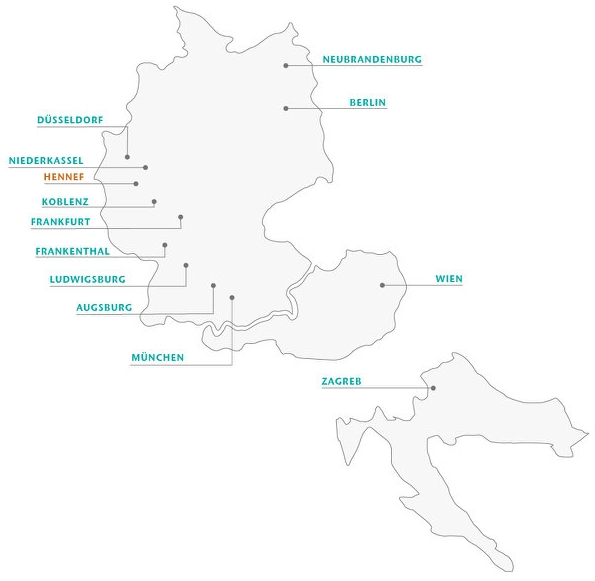
\includegraphics[width = 11cm]{bilder/standorte}
    \caption{Standorte der CONET Technologies Holding GmbH}
\end{figure}

\subsection{Unternehmensstruktur}
Zur Muttergesellschaft CONET Technologies Holdung GmbH gehören acht Tochtergesellschaften. Für die Dauer des Praktikums war die CONET Solutions GmbH mein Arbeitgeber. Diese spezialisiert sich vor allem auf die Entwicklung für von Kunden beauftragte oder für interne Nutzung vorgesehene nicht-standard Software.
\begin{figure}[H]
  \centering
    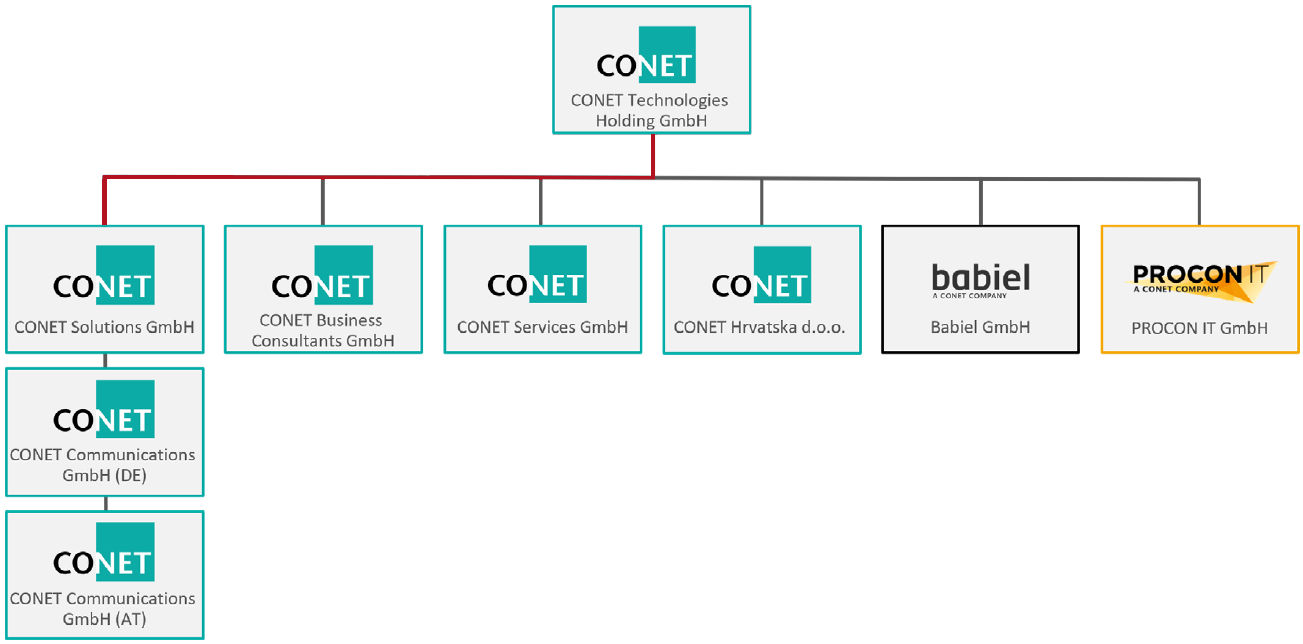
\includegraphics[width = 15cm]{bilder/organigramm_conet}
    \caption{Unternehmensstruktur CONET Technologies Holding GmbH}
\end{figure}

\begin{figure}[H]
  \centering
    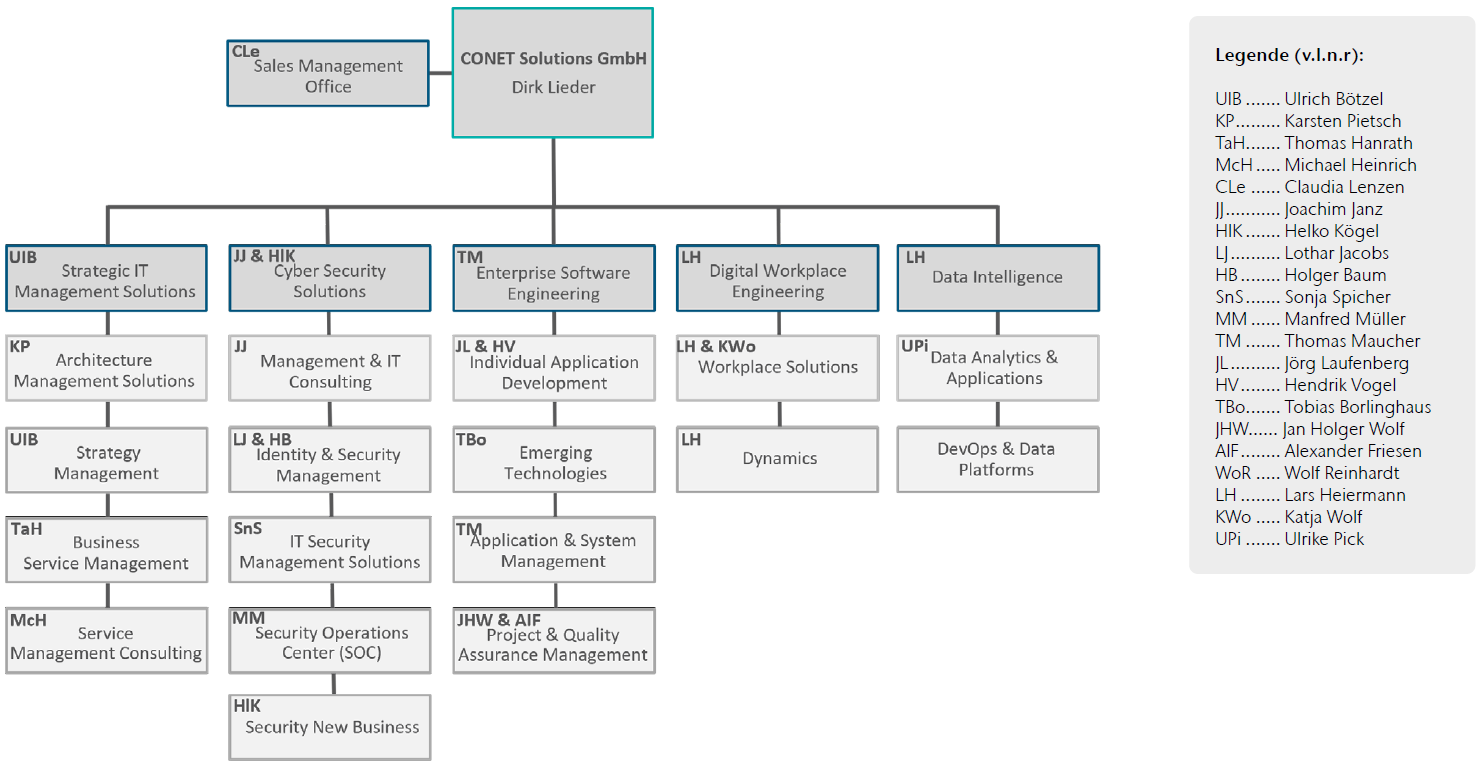
\includegraphics[width = 15cm]{bilder/organigramm_conet_solutions}
    \caption{Unternehmensstruktur CONET Solutions GmbH}
\end{figure}

\subsection{Leistungen}

Die CONET ist ein IT-Beratungsunternehmen, welches in vielen Bereichen Dienstleistungen anbietet. Darunter fallen unter Anderem SAP Consulting, Cyber Security, Cloud Computing, Data Intelligence, Digital Communications \& E-Commerce, Critical Communications, Agile Software Development und Management Consulting. 

\subsection{Kunden}
Die CONET Solutions GmbH ist sowohl im privaten als auch im öffentlich Sektor vertreten. Zu den Kunden gehören die Bundeswehr, Volkswagen, Telekom, Deutsche Bahn und viele weitere. \footcite [Auszug aus der Kundenliste]{Kunden} 